\section{Tóm tắt lý thuyết}
Chương này trình bày bài toán phân lớp nhị phân và thuật toán học Perceptron (Perceptron Learning Algorithm, PLA). 
\subsection{Phân lớp nhị phân}
Bài toán phân lớp nhị phân là phân loại 2 lớp dữ liệu riêng biệt 
(hay còn gọi là binary classification). 

Giả sử có hai class tương ứng hai tập điểm xanh và đỏ,
bài toán đặt ra là từ dữ liệu đã gắn nhãn xanh-đỏ (cho rằng tập 2 dữ liệu này linearly separable), 
ta cần tìm một bộ phân lớp (classifier) có khả năng dự đoán màu của một điểm dữ liệu mới.

\begin{figure}[h]
    \centering
    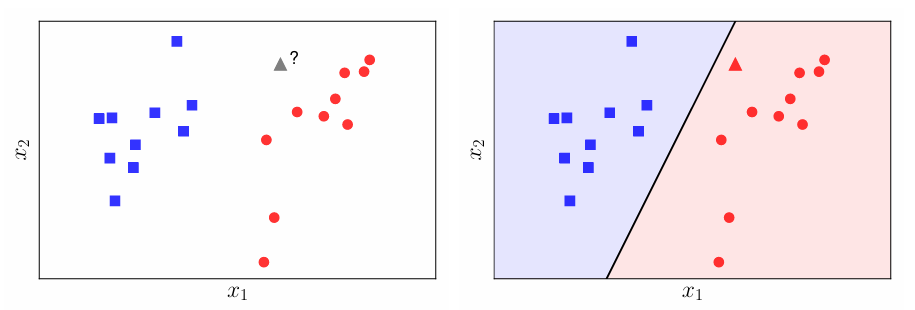
\includegraphics[width=0.5\textwidth]{../images/two-class.png}
    \caption{Bài toán phân lớp nhị phân trong 2D}
\end{figure}

Nếu coi mỗi vector đặc trưng là một điểm trong không gian \(d\) chiều, 
bài toán phân lớp coi như bài toán xác định điểm đó thuộc lớp nào. 
Hay nói cách khác, nếu mỗi lớp chiếm một vùng trong không gian, ta cần xác định
ranh giới (boiundary) giữa các vùng này.

\subsection{Thuật toán perceptron}
\subsubsection{Cách phân lớp}
- Giả sử \(X = [x_1, x_2, \ldots, x_n] \in \mathbb{R}^{d \times N}\) là ma trận vector chứa các điểm huấn luyện.

- \(x_i\) là vector đặc trưng thứ \(i\)

- Nhãn \(y = [y_1, y_2, \ldots, y_n] \in \mathbb{R}^{1 \times N}\)
với \(y_i = 1\) nếu \(x_i\) thuộc lớp 1, \(y_i = -1\) nếu \(x_i\) thuộc lớp 2

Tại một thời điểm, giả sử có boundary là siêu phẳng có pt:
\[
f(\mathbf{x}) = w_1x_1 + \cdots + w_dx_d + w_0
= \mathbf{w}^{T}\mathbf{x} + w_0 = 0
\]

- Với \(\mathbf{w} \in \mathbb{R}^{d}\) là vector hệ số, \(w_0\) là bias (tự do).

- Dùng \textbf{bias trick} để đưa \(w_0\) vào \(\mathbf{w}\), ta có siêu phẳng là

\[
\tilde{\mathbf{x}} = \begin{bmatrix} \mathbf{x} \\ 1 \end{bmatrix}, \qquad
\tilde{\mathbf{w}} = \begin{bmatrix} \mathbf{w} \\ w_0 \end{bmatrix}, \qquad
f(\tilde{\mathbf{x}}) = \tilde{\mathbf{w}}^{T}\tilde{\mathbf{x}} = 0
\]

- Nếu w là nghiệm của bài toán perceptron, với data mới x chưa gán nhãn
, ta có thể gán nhãn bằng cách:
\[
\operatorname{label}(\mathbf{x}) =
\begin{cases}
1 & \text{nếu } \mathbf{w}^{T}\mathbf{x} \ge 0,\\
-1 & \text{o.w.}
\end{cases}
\]

- Nói cách khác, $\operatorname{label}(\mathbf{x}) =
\operatorname{sgn}(\mathbf{w}^{T}\mathbf{x})$ với $\operatorname{sgn}$ là hàm xác định dấu,
giả sử rằng $\operatorname{sgn}(0)=1$.

\subsubsection{Thuật toán phân lớp Perceptron}
Bằng việc xây dựng hàm mất mát:
\[
J(\mathbf{w}) = \sum_{\mathbf{x}_i \in \mathcal{M}}
\left(-y_i \mathbf{w}^{T}\mathbf{x}_i\right)
\]

Trong đó \(\mathcal{M}\) là tập các điểm dữ liệu bị phân lớp lỗi, tức là các điểm dữ liệu mà \(\operatorname{label}(\mathbf{x}_i) \neq y_i\).

Và với một điểm dữ liệu \(x_i\) bị phân lớp lỗi, hàm mất mát và đạo hàm của nó:
\[
J(\mathbf{w}; \mathbf{x}_i, y_i)
= -y_i\mathbf{w}^{T}\mathbf{x}_i,
\qquad
\nabla_{\mathbf{w}}J(\mathbf{w}; \mathbf{x}_i, y_i)
= -y_i\mathbf{x}_i
\]

Và tối ưu hàm mất mát bằng Schoolastic Gradient Descent (SGD):
\[
\mathbf{w} \leftarrow \mathbf{w}
-\eta\left(-y_i\mathbf{x}_i\right)
= \mathbf{w}+\eta y_i\mathbf{x}_i
\]